\documentclass[
  11pt,
  letterpaper,
   addpoints,
   %answers
  ]{exam}

\usepackage{../exercise-preamble}
\usepackage{float}

\begin{document}
\pagestyle{headandfoot}
\firstpagefooter{ }{Página \thepage\ de \numpages}{ }
\runningfooter{ }{Página \thepage\ de \numpages}{ }

\noindent
\begin{minipage}{0.47\textwidth}

\includegraphics[width=\textwidth]{../fcfm_die.png}
\end{minipage}
\begin{minipage}{0.53\textwidth}
\begin{center} 
\large\textbf{Introducción a la Física Moderna} (F1100-5) \\
\large\textbf{Clase auxiliar 4} \\
\normalsize Prof.~ Rodrigo Soto.\\
\normalsize Prof.~Aux.~Erik Sáez - Javiera Toro 
\end{center}
\end{minipage}

\vspace{0.5cm}
\noindent
\vspace{.85cm}

\begin{questions}
%--------------------------
\noindent
\begin{minipage}[t]{0.6\textwidth}
\question Una partícula de masa $m$, después de caer una distancia $h$, se adosa a un resorte (largo) de constante $k$.
El sistema resultante viene gobernado por la ecuación de movimiento
\begin{equation}
  \ddot z + 2\omega_0 \dot z + \omega_0^{2}\, z \;=\; 0,
  \label{eq:crit}
\end{equation}
donde la magnitud $z(t)$ mide la posición de la partícula respecto del punto de equilibrio y
$\omega_0=\sqrt{k/m}$ es la frecuencia natural del sistema. La solución general está dada por
\begin{equation}
  z(t) \;=\; \big(A + B\,t\big)\,e^{-\omega_0 t}.
\end{equation}

\begin{enumerate}
  \item Determine $A$ y $B$ usando las condiciones iniciales.
  \item Sea $t_0$ el instante en que el resorte tiene su máxima compresión. Evalúe $t_0$
  (elija el cero del tiempo en el instante en que la partícula colisiona con el resorte).
  \item Haga un gráfico esquemático de la función $z(t)$.
\end{enumerate}
\end{minipage}\hfill
\begin{minipage}[t]{0.3\textwidth}
  \centering
  \vspace{-1.5\baselineskip}% bajar un poco la imagen
  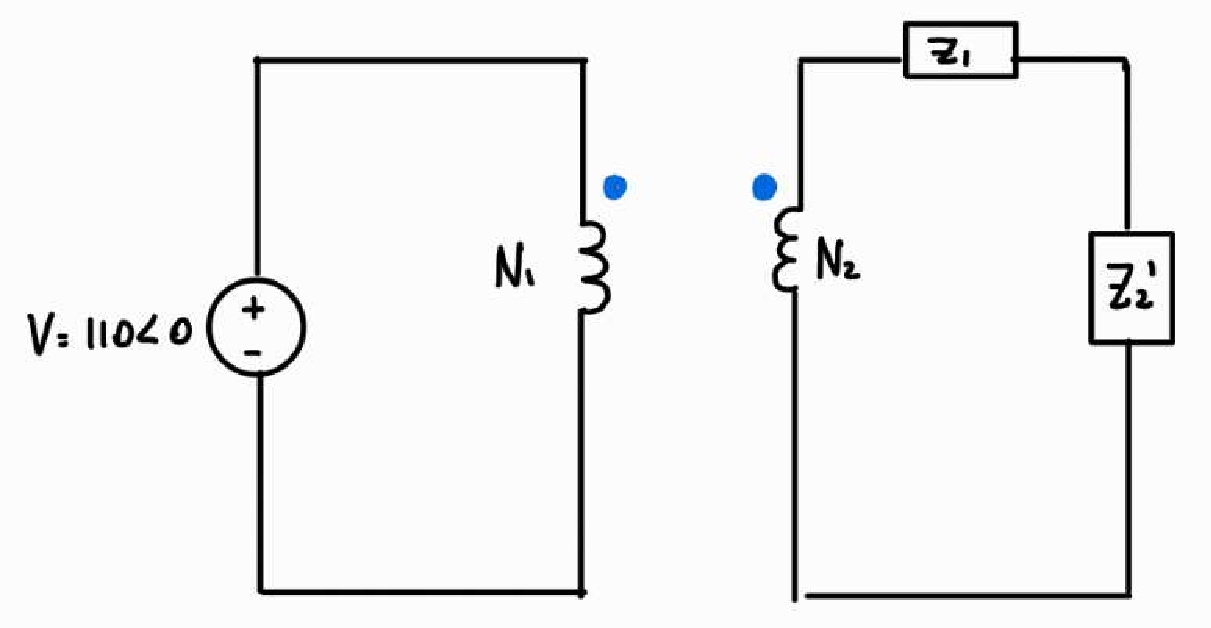
\includegraphics[width=0.8\linewidth]{Auxiliar_2_9}
  \captionsetup{type=figure}
  \captionof{figure}{Partícula que cae sobre un resorte.}
  \label{fig:particula-resorte}
\end{minipage}
%--------------------------
\begin{solution}

\subsection*{Resolución 1.1}

El enunciado entrega la ecuación de movimiento \textbf{respecto del equilibrio} y su solución general:
\begin{align}
m\ddot{z}+2\omega_0\dot{z}+\omega_0^2 z&=0, \qquad \omega_0=\sqrt{\frac{k}{m}},\\
z(t)&=(A+Bt)\,e^{-\omega_0 t}.
\end{align}

Para hallar $A$ y $B$, primero escribimos la ecuación en la coordenada absoluta $y(t)$ (eje positivo hacia arriba), medido desde el piso. Tras el choque, el resorte actúa y el DCL da:
\begin{align}
m\ddot{y}&=-k\big(y-l_0\big)-mg.
\end{align}
El equilibrio estático $y_{\text{eq}}$ se obtiene imponiendo aceleración $\ddot{y}=0 $ y velocidad $\dot{y}=0$ nulas:
\begin{align}
m\cancelto{0}{\ddot{y}}&=-k\big(y_{\text{eq}}-l_0\big)-mg,\\
k\big(y_{\text{eq}}-l_0\big)+mg&=0,\\
y_{\text{eq}}&=l_0-\frac{mg}{k}.
\end{align}
Definimos la coordenada respecto del equilibrio dada por el enunciado:
\begin{align}
z(t)=y(t)-y_{\text{eq}}.
\end{align}

En el instante del choque ($t=0$) el resorte está sin deformación, por lo que $y(t=0)=l_0$. Entonces:
\begin{align}
z(0)=(A - B\cancelto{0}{t})=y(t=0)-y_{\text{eq}}=l_0-\Big(l_0-\frac{mg}{k}\Big)=\frac{mg}{k}
\quad\Longrightarrow\quad
A=\frac{mg}{k}.
\end{align}
La velocidad inicial se obtiene de la caída libre desde altura $h$ (antes del contacto). Usando energía o cinemática:
\begin{align}
mgh=\frac{1}{2}m\,v(0)^2
\quad\Longrightarrow\quad
|v(0)|=\sqrt{2gh}.
\end{align}
Como la partícula llega moviéndose hacia \emph{abajo} y el eje es positivo hacia \emph{arriba}, el signo es:
\begin{align}
\dot z(0)=\dot y(0)=v(0)=-\sqrt{2gh}.
\end{align}
Recordemos que la expresión de $z$ es:
\begin{align}
z(t)&=(A+Bt)e^{-\omega_0 t}.\\
 &= Ae^{-\omega_0 t} + Bte^{-\omega_0 t}.
\end{align}
Luego, tenemos que:
\begin{align}
  \frac{d}{dt}\!\left( A e^{-\omega_0 t}\right) &= -\omega_0 A e^{-\omega_0 t}\\
  \frac{d}{dt}\!\left( B t e^{-\omega_0 t}\right) &= B e^{-\omega_0 t} - \omega_0 B t e^{-\omega_0 t}.
\end{align}
Con lo que, finalmente:
\begin{align}
  \dot z(t) &= -\omega_0 A e^{-\omega_0 t} + B e^{-\omega_0 t} - \omega_0 B t e^{-\omega_0 t}\\
  &= \big(B - \omega_0 A - \omega_0 B t\big)e^{-\omega_0 t}.
\end{align}
De esta manera, tenemos las siguientes ecuaciones relacionadas con la velocidad:
\begin{align}
\dot z(t)&=\big(B-\omega_0A-\omega_0Bt\big)e^{-\omega_0 t},
&
\dot z(0)&=B-\omega_0A.
\end{align}
Luego, imponemos la condición inicial de velocidad. Así, $B$ resulta:
\begin{align}
\dot z(t=0)&= (B - \omega_0 A -\omega_0 B \cancelto{0}{t}) = -\sqrt{2gh}\\
B-\omega_0 A&=-\sqrt{2gh}\\
B&=-\sqrt{2gh}+\omega_0 A\\
B&=-\sqrt{2gh}+g\sqrt{\frac{m}{k}}.
\end{align}
Luego reemplazando las constantes tenemos la solución particular dada por:
\begin{align}
z(t) &= (A + Bt)\,e^{-\omega_0 t},
\end{align}
\begin{align}
z(t) &= \boxed{\left(\frac{mg}{k}+\Big[g\sqrt{\frac{m}{k}}-\sqrt{2gh}\Big]t\right)\,e^{-\sqrt{k/m}\,t}}.
\end{align}
Finalmente, se obtienen las constantes $A$ y $B$.
\subsection*{Resolución 1.2}
La máxima compresión del resorte vendrá dada cuando la velocidad se anule, es decir:
\begin{align}
\dot z(t_0)=0.
\end{align}
Con $z(t)=(A+Bt)e^{-\omega_0 t}$ se tiene
\begin{align}
\dot z(t)&=\big(B-\omega_0A-\omega_0Bt\big)e^{-\omega_0 t},
\end{align}
y, como $e^{-\omega_0 t_0}\neq 0$, tendremos que imponer
\begin{align}
0=B-\omega_0A-\omega_0B\,t_0
\quad\Longrightarrow\quad
t_0=\frac{B-\omega_0A}{\omega_0 B}.
\end{align}
Reemplazando $A$ y $B$ en $t_{0}$ se obtiene
\begin{align}
  t_{0} &= \frac{B - \omega_{0}A}{\omega_{0}B} = \frac{1}{\omega_{0}} - \frac{A}{B}\\
  &= \sqrt{\frac{m}{k}} - \frac{\frac{mg}{k}}{g\sqrt{\frac{m}{k}}-\sqrt{2gh}}\,.
\end{align}
Con esto se determina el instante de máxima compresión del resorte.

\subsection*{Resolución 1.3}
Para analizar la forma de $z(t)$ usamos la solución
\begin{align}
z(t) = (A+Bt)\,e^{-\omega_0 t},\qquad A=\frac{mg}{k},\quad B=\frac{g}{\omega_0}-\sqrt{2gh},\quad \omega_0=\sqrt{\frac{k}{m}}.
\end{align}

Observaciones básicas (consistentes con el gráfico):
\begin{itemize}
  \item Valor inicial independiente de $h$: $\,z(0)=A=\dfrac{mg}{k}$.
  \item Pendiente inicial decreciente con $h$:
  \begin{align}
    \dot z(0)=B-\omega_0 A= -\sqrt{2gh} \;<\; 0.
  \end{align}
  \item Asintóticamente $\lim\limits_{t\to\infty} z(t)=0$ por el factor $e^{-\omega_0 t}$.
\end{itemize}

Todas las curvas parten en $z(0)=mg/k$; a mayor $h$ la pendiente inicial es más pronunciada. Si $h\le h_c$ no hay sobrepaso del equilibrio; si $h>h_c$ hay una compresión máxima en $t_0$ y luego $z(t)$ retorna exponencialmente a $0$.

\begin{figure}[H]
  \centering
  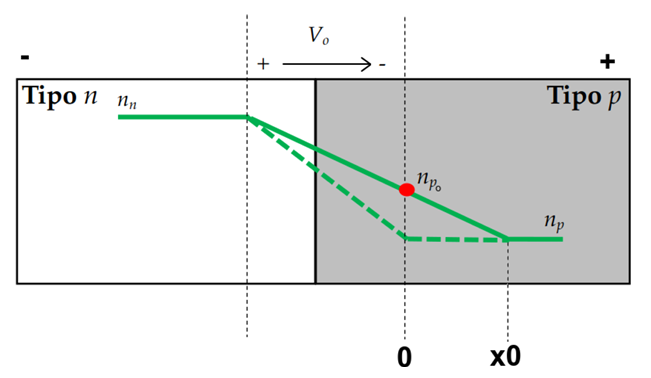
\includegraphics[width=0.7\textwidth]{Auxiliar_2_11}
  \caption{Gráfico esquemático de $z(t)$.}
  \label{fig:grafico-z}
\end{figure}
En el esquema se aprecia el valor inicial $z(0)=mg/k$, la compresión máxima en $t_0$ y el retorno exponencial al equilibrio.
\end{solution}

%--------------------------
\question  Se tiene una cuerda muy larga de tensión $T=1\,\mathrm{N}$ y densidad lineal $\rho=0.25\,\mathrm{kg/m}$.
El extremo izquierdo de la cuerda se mueve de la siguiente forma:
\begin{enumerate}
  \item Está quieto hasta $t=0$.
  \item Desde $t=0\,\mathrm{s}$ hasta $t=2\,\mathrm{s}$, sube con velocidad constante de $1\,\mathrm{cm/s}$.
  \item Luego, se mantiene quieto por $1\,\mathrm{s}$.
  \item Finalmente, baja a velocidad constante hasta la posición inicial, tardando $1\,\mathrm{s}$ en ello.
\end{enumerate}

Grafique el perfil de la onda para $t=3\,\mathrm{s}$.
%--------------------------
\begin{solution}
\subsection*{Resolución 2.}
Buscamos graficar el perfil de la cuerda $y(x,t)$ en $t_f=3~\text{s}$, con $x\ge 0$ y $y$ el desplazamiento vertical (positivo hacia arriba). La cuerda está inicialmente en reposo y horizontal ($y(x,0)=0$), luego tendremos lo siguiente. Usando cm para visualizar amplitudes:

\begin{equation}
y(0,t)=
\begin{cases}
0, & t<0,\\[2mm]
(1~\text{cm/s})\,t, & 0\le t \le 2,\\[2mm]
2~\text{cm}, & 2< t \le 3,\\[2mm]
2~\text{cm}- (2~\text{cm/s})(t-3), & 3< t \le 4,\\[2mm]
0, & t>4.
\end{cases}
\label{eq:y0t}
\end{equation}
Tenemos que tener cuidado con el rango de $3<t\leq 4$ dado que por continuidad debe cumplirse que en t=3 siga siendo 2, por eso se resta 2cm, luego como baja a velocidad constante a su posicion tradando 1s en ello, tenemos que en $t=4$ debe volver a 0, por eso se resta (2 cm/s)(t-3). Esto se visualiza en Fig.~\ref{fig:y0t} muestra $y(0,t)$ (rojo).

\begin{figure}[H]
  \centering
  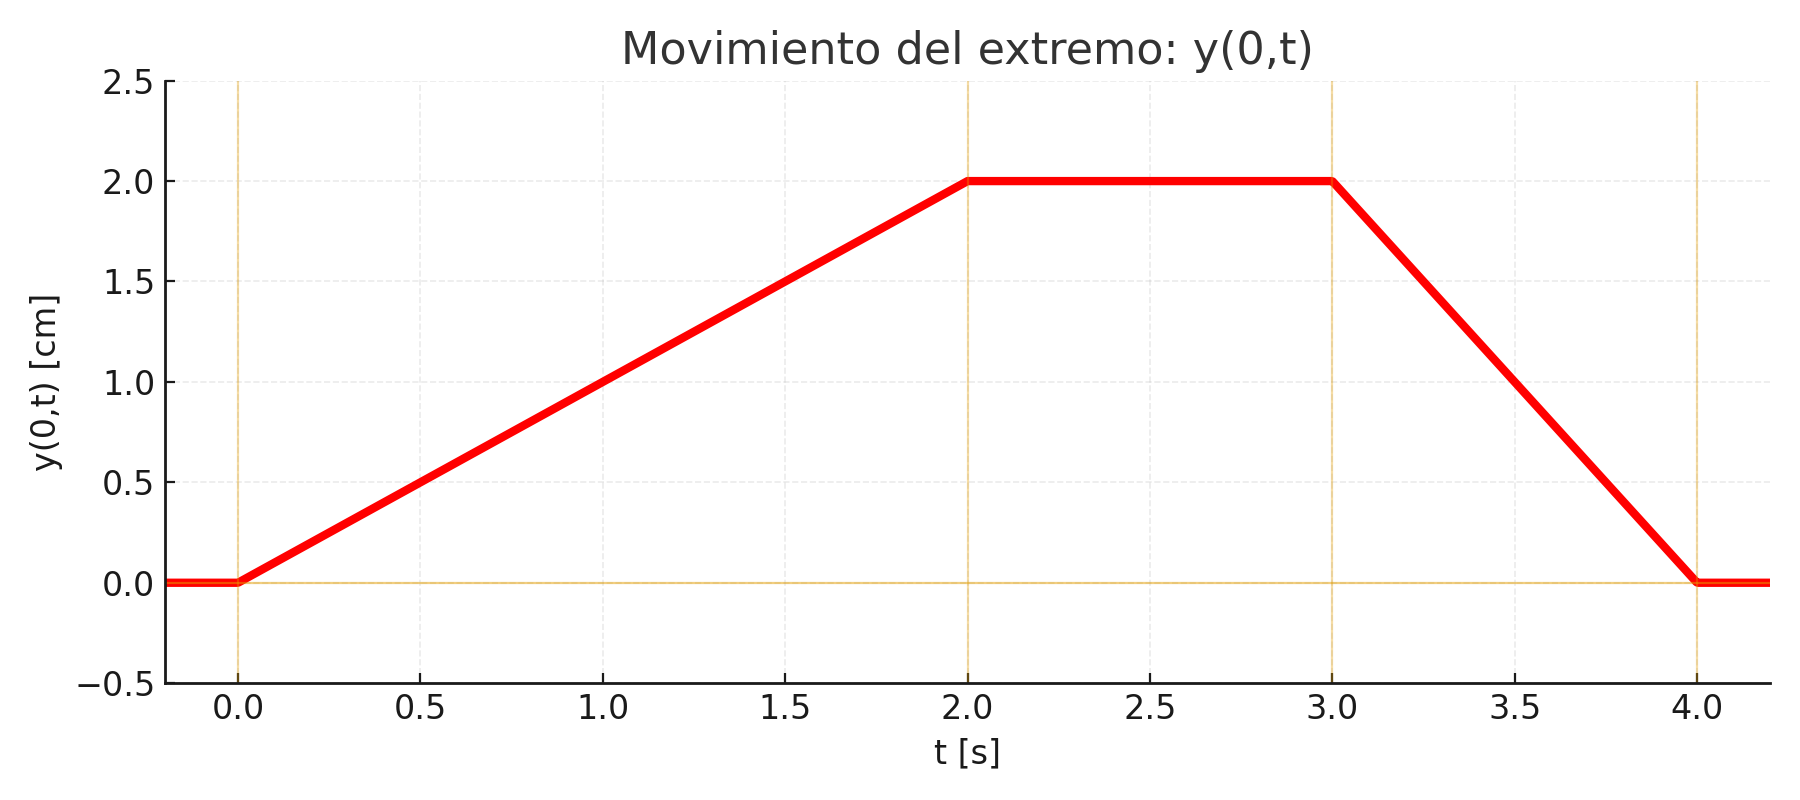
\includegraphics[width=.7\linewidth]{Auxiliar_2_14}
  \caption{Movimiento del extremo: $y(0,t)$ (rojo).}
  \label{fig:y0t}
\end{figure}
Luego tenemos que la velocidad de propagacion de una onda con tensión $T$ y densidad lineal $\rho$, se caracteriza por.
\begin{equation}
c=\sqrt{\frac{T}{\rho}}
=\sqrt{\frac{1~\text{N}}{0.25~\text{kg/m}}}
=2~\text{m/s}.
\label{eq:c}
\end{equation}

Luego para el perfil de la onda es posible caracterizarlo mediante los puntos criticos en $t_f=3~\text{s}$, estos untos seran :
\begin{align}
  (0,0),\quad (2,2),\quad (3,2)
\end{align}
Dado que la onda se mueve con velocidad constante, tenemos que:
\begin{align}
  x_{i}(t=t_f)=x_0+c(t_f-t_i),\quad i=1,2,3,
\end{align}
Donde tenemos que 
\begin{itemize}
  \item $t_{f}$: es el tiempo que queremos graficar $y(x,t_{f})$
  \item $t_{i}$: es el tiempo en que se alcanza el punto critico $i$
\end{itemize}
Por lo tanto tenemos que evaluando por tramos (usando $c=2~\text{m/s}$)
También puede verse mediante ``puntos críticos'' que viajan a velocidad $c$:
\begin{align}
t_1=0 \;\Rightarrow\; x_1=c(3-0)=6~\text{m},\quad & y(x_1,3)=0~\text{cm},\\
t_2=2 \;\Rightarrow\; x_2=c(3-2)=2~\text{m},\quad & y(x_2,3)=2~\text{cm},\\
t_3=3 \;\Rightarrow\; x_3=c(3-3)=0~\text{m},\quad & y(x_3,3)=2~\text{cm},
\end{align}
mientras que el evento en $t_4=4~\text{s}$ aún \emph{no} ha ocurrido para $t_f=3~\text{s}$.
La Fig.~\ref{fig:perfil} muestra el perfil final $y(x,3~\text{s})$ (naranjo).

\begin{figure}[H]
  \centering
  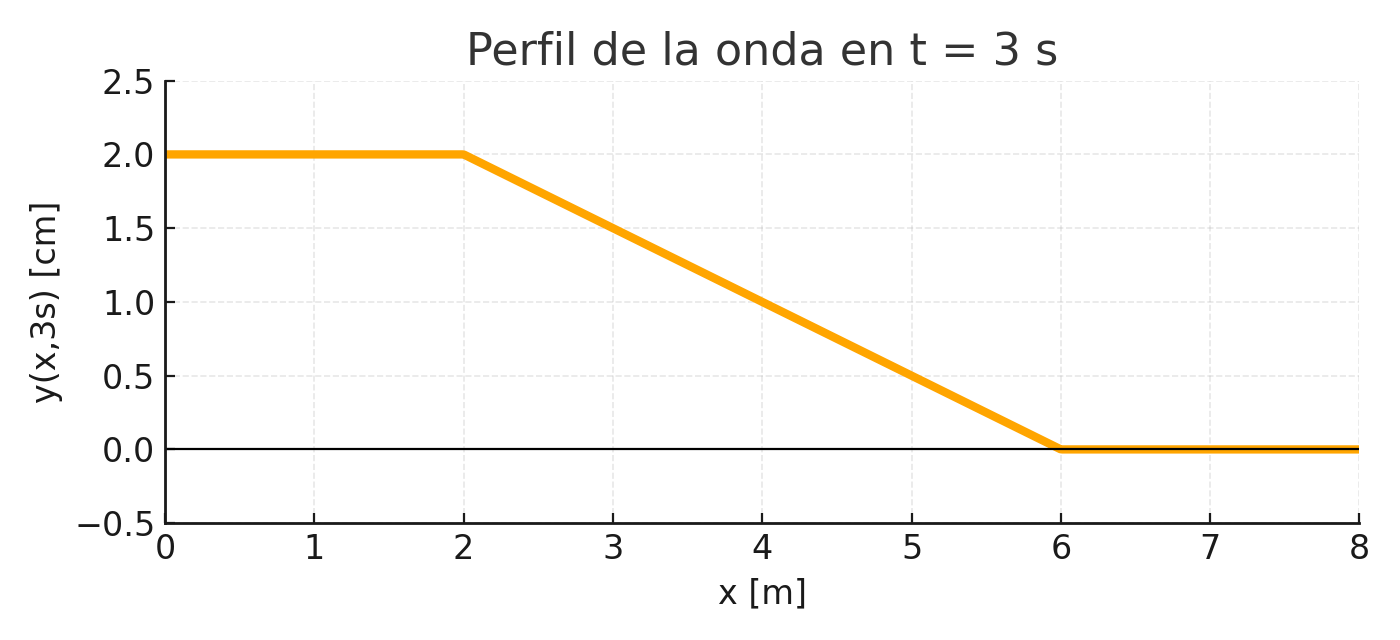
\includegraphics[width=.65\linewidth]{Auxiliar_2_15}
  \caption{Perfil de la onda a $t=3~\text{s}$ (naranjo).}
  \label{fig:perfil}
\end{figure}

\end{solution}

%--------------------------
\question Se tiene una cuerda ideal, sobre la que pasa una onda armónica transversal (el desplazamiento de la cuerda es paralelo al eje $y$ y la onda viaja en el eje $x$). El lado izquierdo (a) de la figura muestra, en función del tiempo, el movimiento de un trozo infinitesimal de la cuerda ubicado en $x=5~\text{m}$.

  \begin{figure}[H]
    \centering
    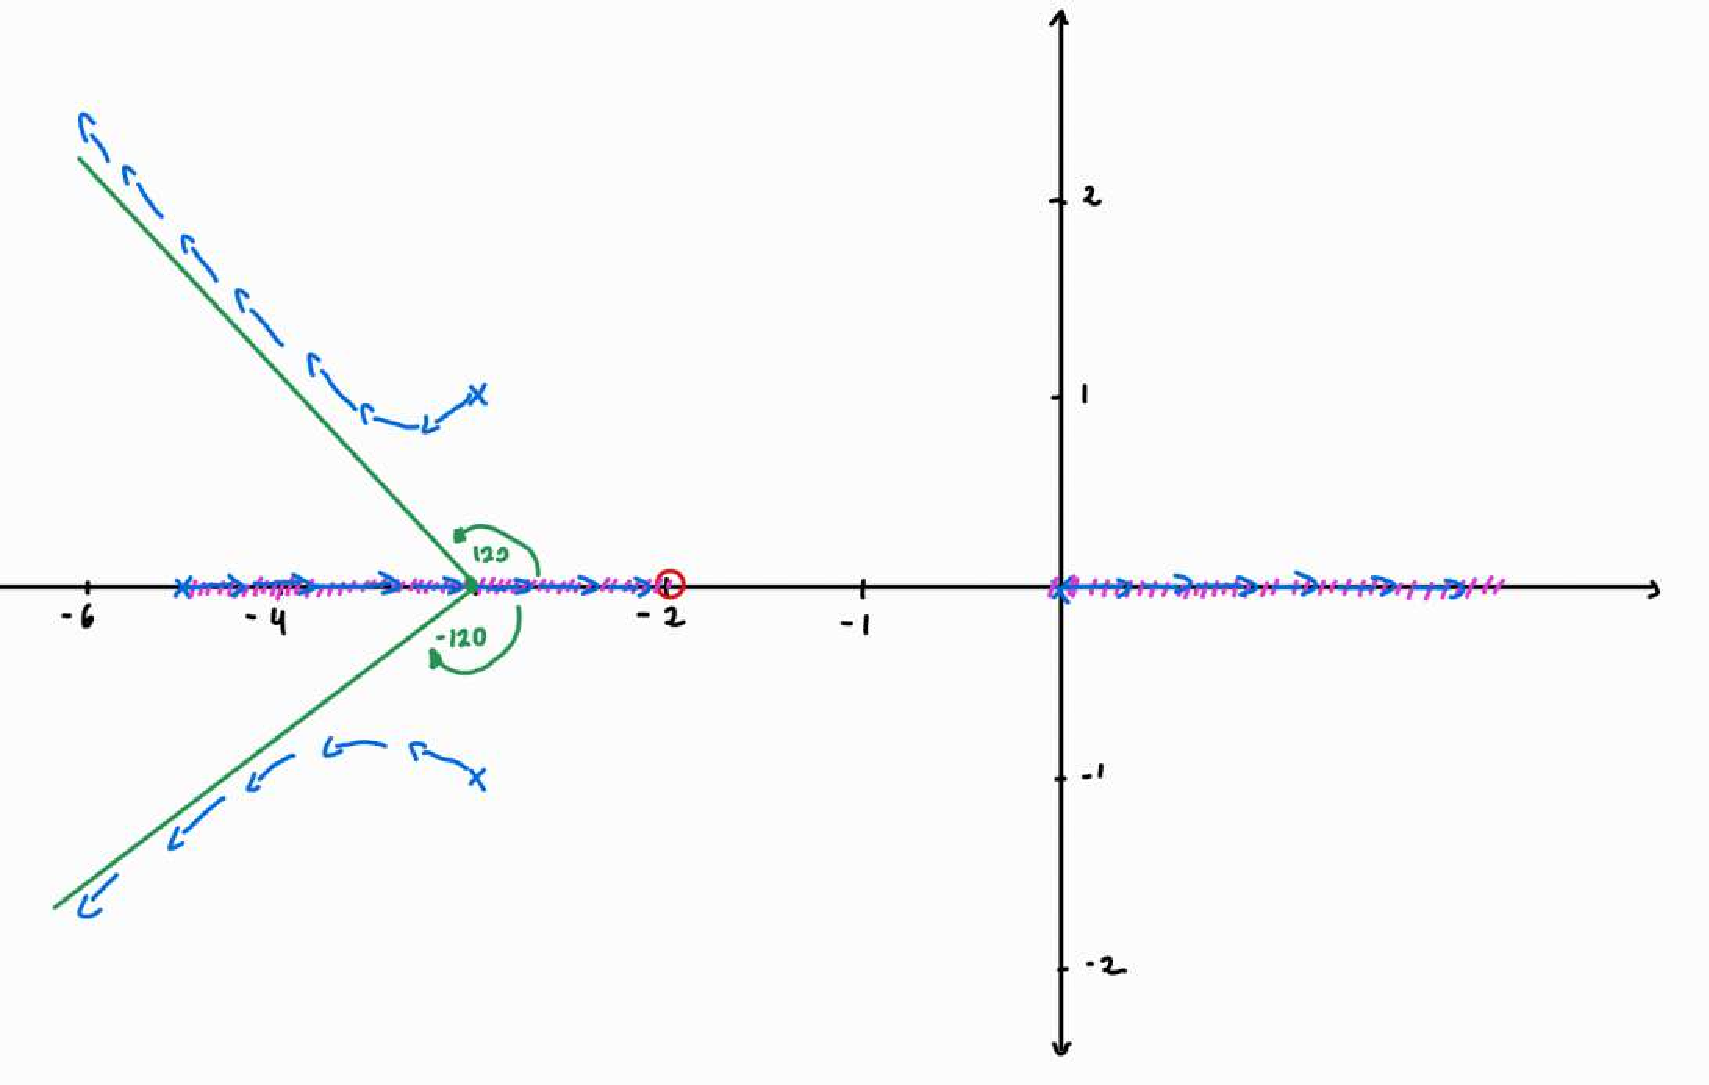
\includegraphics[width=0.75\textwidth]{Auxiliar_2_7}
    \caption{Onda en una cuerda.}
  \label{fig:wave_string}
  \end{figure}
\begin{enumerate}
  \item Uno de los cuatro gráficos de posición $y$ vs.\ $x$ en la parte derecha (b) de la figura representa una \emph{“foto”} de la onda en un instante en el tiempo (el momento en el tiempo para cada caso se indica en el gráfico). Encuentre cuál gráfico $y$ vs.\ $x$ pertenece a la onda mostrada en el lado izquierdo. Justifique su respuesta.

  \item Determine la amplitud, longitud de onda y período de la onda. Explique cómo deduce estos valores.

  \item Encuentre la rapidez a la que viaja la onda.

  \item (\textbf{Propuesto}) Encuentre la dirección (derecha o izquierda) en que se mueve la onda. Justifique su respuesta.
\end{enumerate}
%--------------------------
\begin{solution}
\subsection*{Resolución 2.1}

La figura (a) muestra el movimiento temporal del punto de la cuerda ubicado en $x=5~\text{m}$, es decir, $y(5,t)$. Para decidir cuál de los cuatro perfiles $y(x)$ de (b) corresponde a la misma onda, comparamos valores \textit{puntuales} o puntos críticos de $y$ que se pueden leer con claridad en (a) y verificamos si son consistentes con alguno de los perfiles espaciales de (b) en los tiempos indicados.

\medskip
	\textbf{Paso 1.} Elegimos $t=2~\text{s}$ (dos de los gráficos de (b) están etiquetados con $t=2~\text{s}$). Del gráfico (a) se lee que el punto en $x=5~\text{m}$ cruza el equilibrio:
\begin{equation}
y(x=5,t=2~\text{s}) = 0.
\end{equation}
Entre los perfiles de (b) a $t=2~\text{s}$ (A y C), únicamente el \textbf{gráfico C} tiene $y(5,2~\text{s})=0$. El gráfico A no coincide (en $x=5~\text{m}$ se observa un valor negativo distinto de cero). Para verificar el resto tomamos ahora $t=3~\text{s}$ (gráficos B y D). Del gráfico (a) se lee aproximadamente:
\begin{equation}
y(x=5,t=3~\text{s}) \approx +1.5.
\end{equation}
En los perfiles de (b) a $t=3~\text{s}$, se observa que:
\begin{equation}
\text{en B: } y(x=5,t=3~\text{s})\approx -1.0, 
\qquad
\text{en D: } y(x=5,t=3~\text{s})\approx -1.5,
\end{equation}
ninguno coincide con el valor positivo leído en (a). Por lo tanto, se descartan B y D. Con lo que el único perfil espacial consistente con los datos de (a) es el \textbf{gráfico C}.

\begin{figure}[H]
  \centering
  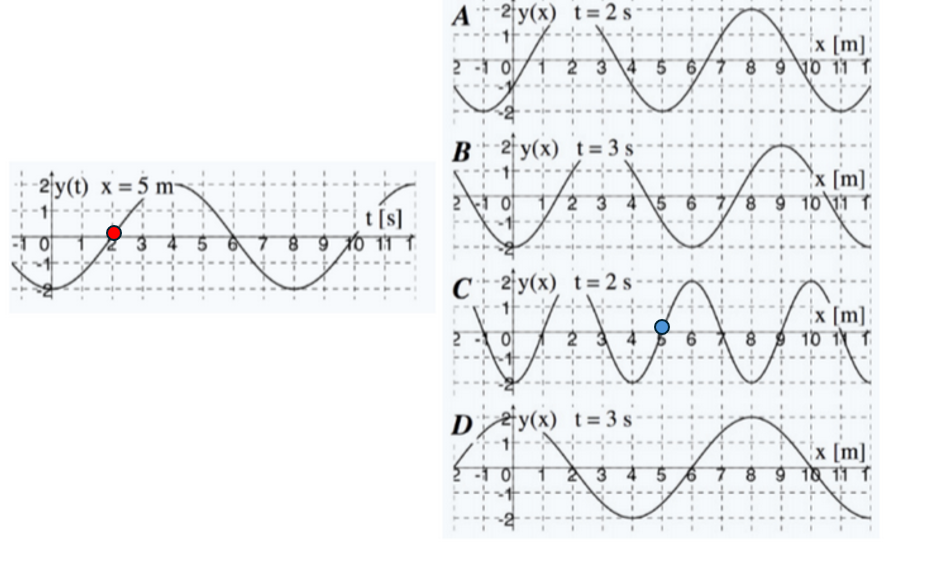
\includegraphics[width=0.8\linewidth]{Auxiliar_2_12}
  \caption{Puntos críticos usados en la comparación: en (a) $y(5,2~\text{s})=0$ (punto rojo) y $y(5,3~\text{s})\approx 1.5$; en (b) solo el gráfico C reproduce $y(5,2~\text{s})=0$ en $x=5~\text{m}$ (punto azul) y es consistente con el descarte de B y D a $t=3~\text{s}$.}
\end{figure}
\subsection*{Resolución 2.2}
Dado que se tienen los gráficos de \(y(x=5,t)\) y \(y(x,2~\text{s})\), es posible leer directamente los parámetros de la onda: período \(T\), longitud de onda \(\lambda\) y amplitud \(A\).

Los cuales se puedendeducen como:
\begin{itemize}
  \item \textbf{Amplitud \(A\)}: desplazamiento máximo respecto del equilibrio (coincide en ambos gráficos).
  \item \textbf{Período \(T\)}: tiempo entre máximos (o mínimos) consecutivos en el gráfico temporal \(y(5,t)\).
  \item \textbf{Longitud de onda \(\lambda\)}: distancia entre mínimos (o máximos) consecutivos en la \emph{“foto”} espacial \(y(x,2~\text{s})\) (panel (b), gráfico C).
\end{itemize}
Dando por tanto los valores de \(A\), \(T\) y \(\lambda\).
\begin{align}
A &= 2, \quad T &= 8~\text{s}, \quad \lambda &= 4~\text{m}.
\end{align}

Graficamente esto se puede observar en la siguiente figura:
\begin{figure}[H]
  \centering
  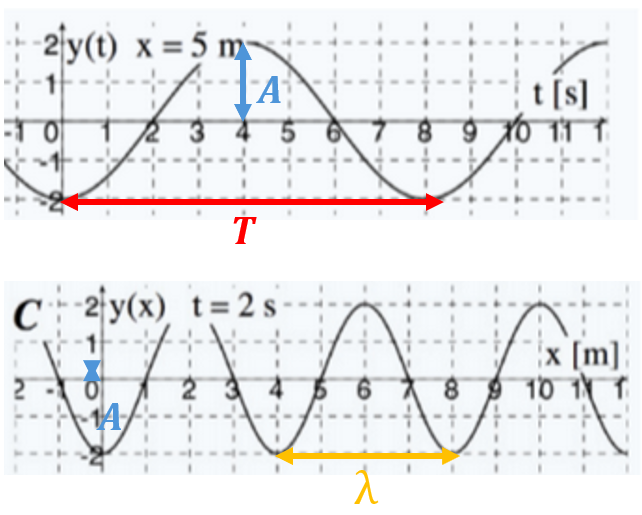
\includegraphics[width=0.5\linewidth]{Auxiliar_2_13}
  \caption{Lectura directa de \(T\) sobre \(y(5,t)\) y de \(\lambda\) sobre \(y(x,2~\text{s})\).
  La amplitud \(A\) es \(2\) en ambos.}
\end{figure}
\subsection*{Resolución 2.3}

Para una onda armónica se cumple lo siguiente:
\begin{equation}
c \;=\; \frac{\omega}{k} \;=\; \frac{\lambda}{T}.
\end{equation}
Con los valores obtenidos en la Sección 2.2,
\begin{align}
\lambda &= 4~\text{m}, &
T &= 8~\text{s},
\end{align}
entonces
\begin{equation}
c \;=\; \frac{\lambda}{T} \;=\; \frac{4~\text{m}}{8~\text{s}}
\;=\; 0.5~\text{m}\,\text{s}^{-1}.
\end{equation}
(De forma equivalente, con \(\omega=\tfrac{2\pi}{T}=\tfrac{\pi}{4}\,\text{rad s}^{-1}\) y
\(k=\tfrac{2\pi}{\lambda}=\tfrac{\pi}{2}\,\text{rad m}^{-1}\),
se tiene \(c=\omega/k=0.5~\text{m s}^{-1}\).)

\subsection*{Resolución 2.4}

Una onda viajera puede escribirse como
\begin{equation}
y(x,t)=f(x\mp ct),
\end{equation}
donde el signo \((-)\) indica propagación hacia la \emph{derecha} y el signo \((+)\) hacia la
\emph{izquierda}. Tomemos como referencia la “foto” espacial a \(t_0=2~\text{s}\):
\begin{equation}
f_0(x):=y(x,2~\text{s}).
\end{equation}
En \(\Delta t=t_1-t_0=2~\text{s}\) (de \(2~\text{s}\) a \(4~\text{s}\)), el patrón se traslada
\begin{equation}
\Delta x = c\,\Delta t = (0.5~\text{m s}^{-1})(2~\text{s}) = 1~\text{m}.
\end{equation}
Luego, para el punto \(x=5~\text{m}\):
\begin{align}
\text{Si viaja a la derecha: } & y(5,4)=f_0(5-\Delta x)=y(4,2),\\
\text{Si viaja a la izquierda: } & y(5,4)=f_0(5+\Delta x)=y(6,2).
\end{align}
Del gráfico temporal \(y(5,t)\) se lee
\begin{equation}
y(5,4~\text{s})\approx +2.
\end{equation}
Mientras que del perfil espacial a \(t=2~\text{s}\) se observa
\begin{equation}
y(4,2)\approx -2, \qquad y(6,2)\approx +2.
\end{equation}
Por lo tanto,
\begin{equation}
y(5,4)=y(6,2)\neq y(4,2)\quad\Rightarrow\quad y(x,t)=f(x+ct),
\end{equation}
lo que implica que la onda \textbf{se propaga hacia la izquierda}.

\end{solution}

%--------------------------
\noindent
\begin{minipage}[t]{0.65\textwidth}
\question Considere una cuerda de densidad lineal $\rho$ y largo $L$ que se cuelga del techo
sin sostener ninguna masa, como se indica en la figura. Se golpea la cuerda en el
centro generando dos pulsos que se propagan, uno ascendente y otro descendente.
\begin{enumerate}
  \item ¿Cuál de los pulsos llegará primero al extremo correspondiente de la cuerda?
  \item Al llegar al respectivo borde, cada pulso será reflejado. Diga si los pulsos se reencontrarán en el centro de la cuerda, por encima o por debajo del mismo. ¿Cómo será la superposición de los pulsos en ese instante?
\end{enumerate}
\end{minipage}\hfill
\begin{minipage}[t]{0.3\textwidth}
  \centering
  \vspace{-1.0\baselineskip}% alinear con el texto
  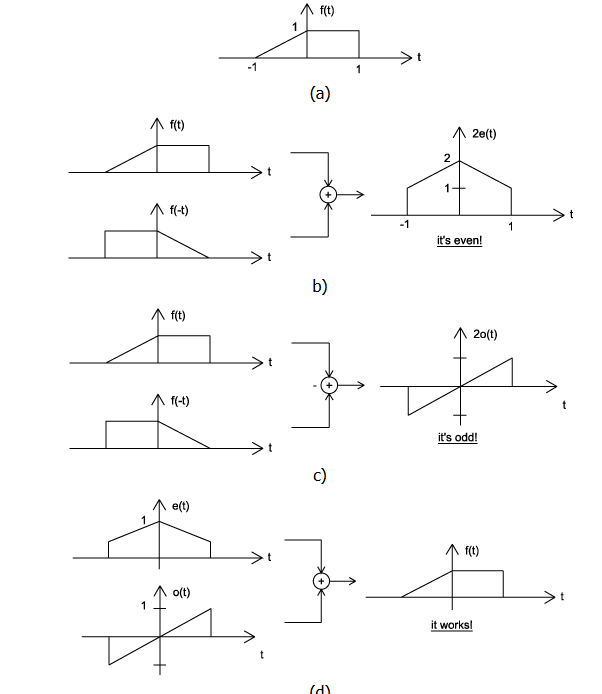
\includegraphics[width=0.95\linewidth]{Auxiliar_2_3}
  \captionsetup{type=figure}
  \captionof{figure}{Cuerda colgante golpeada en el centro: pulsos ascendente y descendente.}
  \label{fig:cuerda-colgante}
\end{minipage}
%--------------------------
\begin{solution}
\subsection*{Resolución 4.1}
Primero, consideremos la rapidez de propagación.
\begin{equation}
  c(z)=\sqrt{\frac{T(z)}{\rho}}.
\end{equation}
donde $T(z)$ es la tensión (que aumenta con la altura $z$) y $\rho$ la densidad lineal. La tensión crece con la altura; véase el esquema:
\begin{figure}[H]
  \centering
  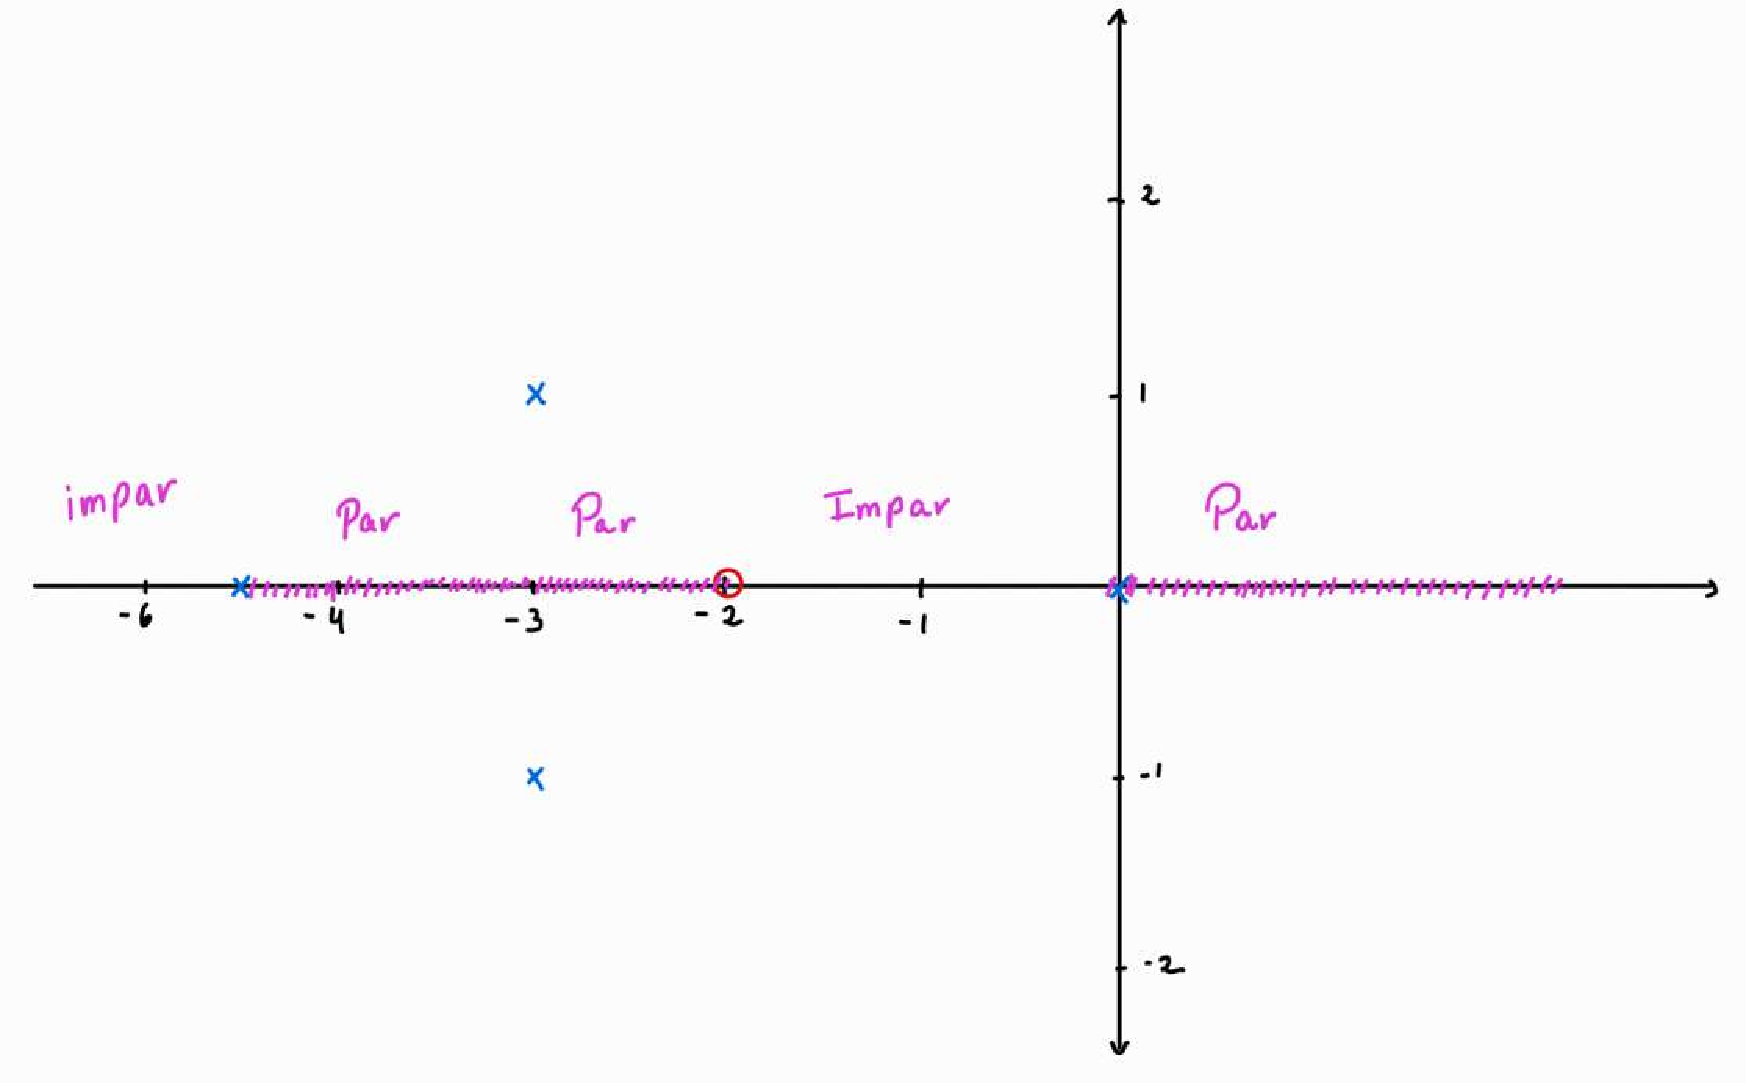
\includegraphics[width=0.6\textwidth]{Auxiliar_2_5}
  \caption{Esquema de la cuerda colgante con tensiones variables.}
  \label{fig:esquema-tension}
\end{figure}
De aquí se observa que, para $z_2>z_1$,
\begin{align}
  T(z_{2}) > T(z_{1}).
\end{align}
Así, cuanto más arriba, mayor tensión y, por tanto, mayor rapidez $c(z)$. El pulso que sube se propaga más rápido que el que baja y, en consecuencia, llega primero a su extremo (el superior).

\subsection*{Resolución 4.2}
Como el pulso que sube viaja más rápido, alcanza antes el techo (extremo fijo) y se refleja con inversión de fase; el pulso que baja llega después al extremo inferior (libre) y se refleja sin inversión. Cuando ambos regresan y se cruzan por primera vez, el pulso superior lleva ventaja temporal, por lo que
\fbox{\textbf{se encuentran por debajo del centro}}. Además, en ese instante tienen signos opuestos (uno invertido y el otro no), de modo que la superposición es \emph{destructiva} (se cancelan momentáneamente).
\end{solution}
%--------------------------
\question Los planetas del sistema solar poseen muchos más tipos de movimientos que el de rotación y el de traslación, algunos de ellos muy complejos, con períodos muy cortos, muy largos o incluso erráticos. Debido a la estabilidad de las órbitas alrededor del Sol, los planetas pueden describir movimientos oscilatorios en el eje radial; es posible ver un ejemplo de esto usando simples aproximaciones.

Se tiene un planeta de masa $m$ que realiza una órbita circular de radio $R_0$ alrededor de una estrella de masa $M$. Considere ahora que la órbita del planeta es ligeramente perturbada, tal que el momento angular de la órbita no cambia, pero sí su radio en una pequeña cantidad. Usando aproximaciones adecuadas, muestre que el radio de la órbita del planeta está descrito por un oscilador armónico.


\begin{figure}[H]
  \centering
  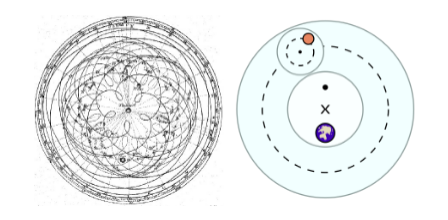
\includegraphics[width=0.5\textwidth]{Auxiliar_2_10}
  \caption{La aproximación realizada en el problema se le llama aproximación epicíclica, este nombre alude a la teoría de los epicilos ideada por los antiguos griegos para explicar los movimientos de los cuerpos celestes bajo el paradigma geocéntrico.}
  \label{fig:epiciclica}
\end{figure}

Asuma que la energia mecanica del sistema está dada por la energía mecánica en coordenadas polares bajo potencial gravitatorio newtoniano:
\begin{equation}
E= \frac{m}{2}\left(r\dot{\theta}\right)^{2} - \frac{mMG}{r}
\end{equation}
y que el momento angular es $L=m r^{2}\dot\theta$.
%--------------------------

\begin{solution}
\subsection*{Resolucion 5.}
Para comenzar el problema, podemos describir la energia del sistema con la energía mecánica en coordenadas polares bajo potencial gravitatorio newtoniano, las cuales vienen dadas por:
\begin{equation}
E= \frac{m}{2}\left(r\dot{\theta}\right)^{2} - \frac{mMG}{r}
\end{equation}
Asumimos un movimiento circular uniforme y escribimos la energia usando el momentum angular $L=m r^{2}\dot\theta$, por lo tanto
\begin{equation}
E = \frac{L^{2}}{2mR^{2}} - \frac{GMm}{R}
\end{equation}

Ahora consideraremos la perturbacion dada para lo cual se realiza el cambio de variables convenientes dados por
\begin{equation}
r(t)=R_0+x(t), \qquad |x|\ll R_0, \qquad \dot r=\dot x.
\end{equation}
donde $R_0$ es el radio de la órbita circular no perturbada y $x(t)$ es la pequeña perturbación en el radio, por eso se puede considerar que $|x|\ll R_0$, luego reescribiendo la energia se tiene que:
\begin{equation}
E \;=\; \frac{m}{2}\,\dot x^{2}
\;+\; \frac{L^{2}}{2m\,(R_0+x)^{2}}
\;-\; \frac{GMm}{R_0+x}.
\label{eq:Eexpandstart}
\end{equation}
Nuestro objetivo principal es buscar la forma del oscilador armónico en función de $x \rightarrow U = \frac{1}{2}kx^{2}$, para ello buscamos reordenar los términos que corresponde a x:
\begin{align}
  E= \frac{m}{2}\,\dot x^{2} + \frac{1}{(R_{0}+x)^{2}}\left(\frac{L^{2}}{2m} - mMG(R_{0}+x)\right)
\end{align}
Dado que tenemos un termino cuadratico, es posible realizar una expansion de Taylor en $\frac{1}{(R_0+x)^{2}}$:
\begin{align}
\frac{1}{R_0+x}
&= \frac{1}{R_0}\left(1-\frac{x}{R_0}+\frac{x^{2}}{R_0^{2}}-\frac{x^{3}}{R_0^{3}}+\cdots\right),\\[2mm]
\frac{1}{(R_0+x)^{2}}
&= \frac{1}{R_0^{2}}\left(1-\frac{2x}{R_0}+\frac{3x^{2}}{R_0^{2}}-\frac{4x^{3}}{R_0^{3}}+\cdots\right).
\end{align}
Como $|x|/R_0\ll 1 \rightarrow \frac{x}{R_{0} }\ll 1$, podemos descartar los terminos de orden 2 y mayores para aproximar \eqref{eq:Eexpandstart}:
\begin{align}
  \frac{1}{(R_0+x)^{2}} &\approx \frac{1}{R_0^{2}}\left(1-\frac{2x}{R_0}\right),\\[2mm]
\end{align}
De esta manera la energia quedara como:
\begin{align}
  E= \frac{m}{2}\,\dot x^{2} +\frac{1}{R_0^{2}}\left(\frac{L^{2}}{2m} - mMG(R_0)\right)
\end{align}
Nos queda molestando el termino con el momento angular L, pero tenemos que tener en cuenta las propiedades del movimiento circular uniforme antes de la perturbacion, como L se mantuvo constante no hay problemas con suar el movimiento circular uniforme para definirlo
\begin{align}
  ma_{c} = \frac{mMG}{R_{0}^{2}} \quad a_{c} = R_{0}\Omega_{0}^{2}
\end{align}
Con lo que tenemos que:
\begin{align}
  mR_{0}\dot{\theta}^{2} &= \frac{mMG}{R_{0}^{2}} / \cdot \frac{mR_{0}^{3}}{mR_{0}^{3}}
  \frac{m^{2}R_{0}^{4}\dot{\theta}^{2}}{mR_{0}^{3}} &= \frac{GMm}{R_{0}^{2}}\\
  L^{2} &= GMm^{2}R_{0}\\
\end{align}
De esta manera es posible obtener $L$; luego podemos reemplazarlo en la energía, obteniendo
\begin{align}
E &= \frac{m}{2}\,\dot x^{2}
 + \frac{1}{R_0^{2}}\Big(1-\frac{2x}{R_0}\Big)\Big[\frac{GMm\,R_0}{2} - GMm\,(R_0 + x)\Big] \\
\Leftrightarrow\quad
E &= \frac{m}{2}\,\dot x^{2}
 + \frac{1}{R_0^{2}}\Big(1-\frac{2x}{R_0}\Big)\Big[-\frac{GMm\,R_0}{2} - GMm\,x\Big] \\
\Leftrightarrow\quad
E &= \frac{m}{2}\,\dot x^{2}
 + \Big(-\frac{GMm}{2R_0}\Big)\Big(1-\frac{2x}{R_0}\Big)\Big(1+\frac{2x}{R_0}\Big).
\end{align}

Finalmente, la energía adopta la forma de un oscilador armónico:
\begin{equation}
E \,=\, \frac{m}{2}\,\dot x^{2} \,+\, \frac{1}{2}\,\underbrace{\left(\frac{4\,GMm}{R_0^{3}}\right)}_{\displaystyle k}\,x^{2} \, - \, \frac{GMm}{2R_0}.
\end{equation}
Nombramos \(k = \tfrac{4\,GMm}{R_0^{3}}\), de modo que la energía total queda
\begin{equation}
E \,=\, \frac{m}{2}\,\dot x^{2} \,+\, \frac{1}{2}\,k\,x^{2} \, - \, \frac{GMm}{2R_0}.
\end{equation}
A partir de esto se deduce que \(x\) satisface la ecuación de movimiento
\begin{equation}
m\,\ddot x \,=\, -\,k\,x,
\end{equation}
cuya solución general es
\begin{equation}
x(t) \,=\, A\,\sin\!\left(\sqrt{\tfrac{k}{m}}\,t + \phi_0\right).
\end{equation}
Observación: el término constante \(-\tfrac{GMm}{2R_0}\) corresponde a la energía del movimiento circular inicial sin perturbación.


\end{solution}

\end{questions}
\end{document}